\documentclass[a4paper,12pt]{article}

%%% Размер шрифта
\usepackage[14pt]{extsizes}

%%% Поля
\usepackage[
	left=2cm,
	right=2cm,
	top=2cm,
	bottom=3cm,
	bindingoffset=0cm
]{geometry}

%%% Работа с русским языком
\usepackage{cmap}						% поиск в PDF
\usepackage{mathtext}					% русские буквы в формулах
\usepackage[T2A]{fontenc}				% кодировка
\usepackage[utf8]{inputenc}				% кодировка исходного текста
\usepackage[english,russian]{babel}		% локализация и переносы
\usepackage{indentfirst}
\frenchspacing

%%% Дополнительная работа с математикой
\usepackage{amsmath,amsfonts,amssymb,amsthm,mathtools}  % AMS

%%% Текст в колонки
\usepackage{multicol}

%%% Списки
\usepackage{enumitem}
\setlist{nosep, leftmargin=*}
\renewcommand{\labelenumi}{\arabic*)}

%%% Системы уравнений
\usepackage{cases}

%%% Таблицы
\usepackage{array}

%%% Рисунки
\usepackage{graphicx}
\usepackage{float}

%%% Точка в подписях к рисункам
\usepackage[labelsep=period]{caption}

%%% Список литературы
\bibliographystyle{bibliography_style/gost-numeric.bbx}
\usepackage[
	natbib = true,
	style = gost-numeric,
	sorting = none,
	backend = biber,
	language = autobib,
	autolang = other
]{biblatex}
\addbibresource{references.bib}

%%% Исправление символа номера при использовании gost-numeric.bbx
\usepackage{textcomp}
\DefineBibliographyStrings{russian}{number={\textnumero}}

%%% Гиперссылки
\usepackage[pdftex,unicode]{hyperref}

%%% Перенос знаков в формулах (по Львовскому)
\newcommand*{\hm}[1]{#1\nobreak\discretionary{}{\hbox{$\mathsurround=0pt #1$}}{}}


%%% Свои команды

\newcommand*{\No}{\textnumero}

\newcommand{\vect}[1]{\boldsymbol{#1}}
\newcommand{\vx}{{\vect{x}}}
\newcommand{\vn}{{\vect{n}}}
\newcommand{\vrho}{{\vect{\rho}}}

\newcommand{\aver}[1]{\widetilde{#1}}
\newcommand{\avphi}{{\aver{\phi}}}
\newcommand{\avpsi}{{\aver{\psi}}}
\newcommand{\avlaplphi}{{\aver{\Delta \phi}}}

\newcommand{\ga}{{g^{(a)}}}
\newcommand{\gb}{{g^{(b)}}}

\newcommand{\half}{\cfrac{1}{2}}

\newcommand{\partderiv}[2]{\cfrac{\partial #1}{\partial #2}}
\newcommand{\partsecondderiv}[2]{\cfrac{\partial^2 #1}{\partial {#2}^2}}
\newcommand{\partt}[1]{\partderiv{#1}{t}}
\newcommand{\partx}[1]{\partderiv{#1}{x}}
\newcommand{\partxx}[1]{\partsecondderiv{#1}{x}}
\newcommand{\partvn}[1]{\partderiv{#1}{\vn}}
\newcommand{\partr}[1]{\partderiv{#1}{r}}
\newcommand{\partrr}[1]{\partsecondderiv{#1}{r}}

\newcommand{\partflderiv}[2]{\partial #1 / \partial #2}
\newcommand{\partflsecondderiv}[2]{\partial^2 #1 / \partial {#2}^2}
\newcommand{\partflt}[1]{\partflderiv{#1}{t}}
\newcommand{\partflx}[1]{\partflderiv{#1}{x}}
\newcommand{\partflxx}[1]{\partflsecondderiv{#1}{x}}
\newcommand{\partflvn}[1]{\partflderiv{#1}{\vn}}
\newcommand{\partflr}[1]{\partflderiv{#1}{r}}
\newcommand{\partflrr}[1]{\partflsecondderiv{#1}{r}}

\newcommand{\scalsq}[1]{\left( \nabla #1, \nabla #1 \right)}

\newcommand{\norm}[1]{\| \, #1 \, \|}
\newcommand{\enorm}{{\| \cdot \|}}

\newcommand{\plapl}[2]{\Div(\norm{\nabla #1}_2^{#2} \nabla #1)}
\newcommand{\bilapl}[1]{\Delta^2 #1}

\newcommand{\intt}{{\int\limits_{t_j}^{t_{j + 1}}}}
\newcommand{\intOmega}{{\int\limits_{\Omega_i}}}

\newcommand{\gridfunc}[1]{\left[ \cfrac{\partial #1}{\partial r} \right]}
\newcommand{\gridpartphi}{{\gridfunc{\phi}}}
\newcommand{\gridpartlaplphi}{{\gridfunc{(\Delta \phi)}}}

\newcommand{\Natural}{{\mathbb{N}}}
\newcommand{\Real}{{\mathbb{R}}}
\newcommand{\bigO}{{\mathcal{O}}}
\newcommand{\clOmega}{{\overline{\Omega}}}

\newcommand{\anylimits}{{\bigg|_{...}^{...}}}

\newcommand{\tpoint}{{\text{.}}}
\newcommand{\tcomma}{{\text{,}}}
\newcommand{\tsemicolon}{{\text{;}}}

\newcommand{\forcehyphenation}{-\linebreak}

\newcommand{\multeqstart}{
	\begingroup
	\setlength{\abovedisplayshortskip}{\the\abovedisplayskip}
	\setlength{\belowdisplayshortskip}{\the\belowdisplayskip}
}
\newcommand{\multeqnext}{
	\vspace{-7mm}
}
\newcommand{\multeqfinish}{
	\endgroup
}


%%% Свои операторы
\DeclareMathOperator{\Div}{{div}}


%%% Оформление теорем

\theoremstyle{plain}
\newtheorem{theorem}{Теорема}
\newtheorem{proposition}{Утверждение}

\theoremstyle{remark}
\newtheorem{remark}{Замечание}


%%% Пояснение к меткам
% eq	-- equation
% cond	-- condition
% char	-- characteristic
% sch	-- scheme
% est	-- estimation
% exp	-- experiment
% fig	-- figure
% tab	-- table
% sec	-- section
% ssec	-- subsection


%%% Описание препринта
\newcommand{\PreprintTitle}{%
	Численное исследование обобщения модели развития канала электрического пробоя типа <<диффузной границы>>%
}
\newcommand{\PreprintTitleFormatted}{
	Численное исследование обобщения \\ модели развития канала электрического пробоя \\ типа <<диффузной границы>>
}
\newcommand{\PreprintTitleEnglish}{%
	Numerical analysis of a generalized diffuse interface model for the electrical breakdown process%
}
\newcommand{\PreprintAuthors}{%
	А.~С.~Пономарев, Е.~В.~Зипунова, Е.~Б.~Савенков%
}
\newcommand{\PreprintAuthorsEnglish}{%
	A.~S.~Ponomarev, E.~V.~Zipunova, E.~B.~Savenkov%
}


%%%%%%%%%%%%%%%%%%%%%%%%%%%%%%%%%%%%%%%%%%%%%%%%%%%%%%%%%%%%%%%%%%%%%%%%%%%%%%%%

\begin{document}

%%%%%%%%%%%%%%%%%%%%%%%%%%%%%%%%%%%%%%
\begin{titlepage}

\begin{center}
	РОССИЙСКАЯ АКАДЕМИЯ НАУК \\
	ОРДЕНА ЛЕНИНА \\
	ИНСТИТУТ ПРИКЛАДНОЙ МАТЕМАТИКИ \\
	имени М. В. КЕЛДЫША \\

	\vspace*{60mm}
	{
		\Large{\PreprintAuthors} \\
	}
	\vspace*{20mm}
	{
		\large \textbf{\PreprintTitleFormatted} \\
	}
	\vspace*{110mm}
	\Large{Москва, 2024}
	\vspace*{-50mm}
\end{center}

\end{titlepage}
%%%%%%%%%%%%%%%%%%%%%%%%%%%%%%%%%%%%%%%

\setcounter{page}{2}

\thispagestyle{empty}

\noindent \emph{\PreprintAuthors,} \PreprintTitle \\[3mm]
\textbf{Аннотация} \\
{
	\small
	В настоящей работе проводится численное исследование ранее предложенного обобщения модели типа диффузной границы, описывающей развитие канала электрического пробоя в твердом диэлектрике. Для этого ищется стационарное распределение фазового поля в нескольких характеристических случаях задачи. При построении разностной схемы применена модификация метода конечных объемов, так что схема позволяет задать граничные условия на множествах высшей коразмерности в трехмерном пространстве, притом что у решения задачи в точках этих множеств допускается особенность. \\[3mm]
	\textbf{Ключевые слова:} модель типа диффузной границы, фазовое поле, метод конечных объемов, электрический пробой \\[5mm]
}
\begin{otherlanguage}{english}
\emph{\PreprintAuthorsEnglish,} \PreprintTitleEnglish \\[3mm]
\textbf{Abstract} \\
{
	\small
	The subject of the present work is a previously suggested generalization of a diffuse interface model describing the development of an electrical breakdown channel in a solid dielectric. Numerical analysis for the model is performed. In the analysis, the stationary distribution of the phase field is found in several characteristic cases of the problem. A modification of the finite volume method is applied so that the numerical scheme is available for determining the boundary conditions at sets of higher codimension in three-dimensional space. At that the solution function is expected to have a singularity at the points of these sets. \\[3mm]
	\textbf{Key words and phrases:} diffuse interface model, phase field, finite volume method, electrical breakdown \\[5mm]
}
\end{otherlanguage}

\clearpage

%!TEX root = ../main.tex

\section{Введение}

Электрический пробой~-- это явление резкого возрастания тока в диэлектрике при приложении электрического напряжения выше некоторого критического значения. Механизм разрушения диэлектрика под действием электрического поля сложен и многообразен: оно может иметь различные причины, характер развития, сопутствующие физические процессы \cite{vorobiev_dielectric_physics}.

Среди многообразия математических моделей, созданных для описания развития канала электрического пробоя, выделим предложенную в работе \cite{pitike_dielectric_breakdown} модель типа диффузной границы.

В настоящее время модели типа диффузной границы составляют целый класс подходов для решения задач в различных областях науки и техники. В частности, описанная в работе \cite{pitike_dielectric_breakdown} модель построена как формальное обобщение ранее известных моделей типа диффузной границы, применяемых в теории трещин.

Исследование и дальнейшее развитие упомянутой модели можно найти в работах \cite{zipunova_higher_codimension, zipunova_conservative, zipunova_thermomechanical, ponomarev_stability}. Основные положения метода диффузной границы в применении к моделированию развития канала электрического пробоя перечислены в работе \cite{ponomarev_stability}.

Модели типа диффузной границы используются для описания систем, в которых вещество может находиться в нескольких различных состояниях~-- фазах,~-- причем вещество в одной и той же фазе образует некоторые однородные области. В моделях типа диффузной границы распределение фаз вещества задается гладкой функцией $\phi$~-- фазовым полем,~-- которая в каждой области однородности близка к постоянной. Характерная толщина разделяющего слоя (<<диффузной границы>>) и, соответственно, скорость изменения~$\phi$ при переходе от одной фазы к другой определяется параметрами модели.

В работе \cite{zipunova_higher_codimension} проводится исследование свойства упомянутой модели развития канала электрического пробоя, которое можно назвать коразмерностью <<включений>>. Для задач теории трещин естественным будет двумерное включение (плоская трещина) в трехмерной среде вещества~-- в таком случае говорят, что коразмерность объекта равна 1. Обратим внимание, что, хотя исследуемая модель, как было сказано, получена на основе моделей из теории трещин, для нее характерным будет одномерное включение (канал пробоя), то есть имеющее коразмерность 2. В работе \cite{zipunova_higher_codimension} указано, что это может привести к нетривиальным последствиям, и предложено определенное обобщение исходной модели, которое предположительно делает ее более адекватной.

Суть обобщения состоит в формальном добавлении в уравнения модели двух слагаемых высших порядков с некоторыми коэффициентами. Целью настоящей работы является численная проверка поведения модели при различных значениях коэффициентов. Для этого ищется стационарное распределение фазового поля $\phi$ в нескольких характеристических случаях. Построение разностной схемы для задачи несет определенные сложности, связанные с необходимостью задать граничные условия на множествах коразмерности~2 и~3 в трехмерном пространстве. Предполагается, что точках этих множеств функция фазового поля $\phi$ имеет особенность.

Авторами применена модификация метода конечных объемов. Для части конфигураций обобщенной модели она позволила составить разнотную схему. Создана компьютерная программа, реализующая схему; проделаны расчеты, их результаты приведены в виде графиков. Для остальных конфигураций модели в процессе применения метода возникли фундаментальные проблемы, что позволяет выдвинуть гипотезу о некорректной постановке дифференциальной задачи в этих случаях.

%!TEX root = ../main.tex

\section{Постановка задачи и модель}
\label{sec:problem_and_model}

Приведем краткое описание математической модели, предложенной в работе \cite{pitike_dielectric_breakdown}. Подробное описание модели и физического смысла ее уравнений и параметров можно найти в работе \cite{ponomarev_stability}.

Рассматривается ограниченная область пространства $\Omega \subset \Real^3$. Распределение фаз вещества в ней задается гладкой функцией $\phi: \Omega \times [0, +\infty)_t \hm \to [0, 1], \; \phi(\vx, t)$~-- фазовым полем; вещество может находиться в одной из двух фаз: $\phi \approx 1$~-- <<неповрежденное>>, $\phi \approx 0$~-- <<полностью разрушенное>> (то есть относящееся к каналу пробоя),~-- а также в промежуточных состояниях в зоне диффузной границы.

Диэлектрическую проницаемость среды $\epsilon$ предлагается описать следующей формулой:
\begin{equation}
	\epsilon(\vx, t) = \epsilon[\phi] = \cfrac{\epsilon_0(\vx)}{f(\phi(\vx, t)) + \delta} \tpoint
	\label{eq:epsilon}
\end{equation}
Здесь $\epsilon_0(\vx)$~-- диэлектрическая проницаемость неповрежденной среды, $f(\phi) \hm = 4\phi^3 - 3\phi^4$~-- интерполирующая функция, $0 < \delta \ll 1$~-- регуляризующий параметр.

Помимо фазового поля $\phi$, состояние системы описывает также функция $\Phi: \Omega \times [0, +\infty)_t \to \Real, \; \Phi(\vx, t)$~-- потенциал электрического поля.

Постулируется следующее выражение для свободной энергии системы $\Pi$:
\begin{gather*}
	\Pi = \int \limits_\Omega \pi d \vx \tcomma \\
	\pi = -\half \epsilon[\phi] \scalsq{\Phi} + \Gamma \cfrac{1 - f(\phi)}{l^2} + \cfrac{\Gamma}{4} \scalsq{\phi} \tpoint
\end{gather*}
Здесь $\Gamma > 0, \; l > 0$~-- числовые параметры модели, константы.

Постулируются два уравнения, определяющие динамику системы:
\begin{equation*}
\begin{cases}
	\cfrac{\delta \Pi}{\delta \Phi} = 0 \tsemicolon \\[3mm]
	\cfrac{1}{m} \partt{\phi} = -\cfrac{\delta \Pi}{\delta \phi} \tpoint
\end{cases}
\end{equation*}
Здесь константа $m > 0$~-- числовой параметр модели, называемый подвижностью. Говоря нестрого, согласно первому уравнению электрический потенциал $\Phi$ распределяется так, чтобы свободная энергия была минимальной; согласно второму~-- фазовое поле $\phi$ с определенной скоростью стремится к тому, чтобы свободная энергия была минимальной.

Отыскав явно вариационные производные в двух уравнениях выше, получим следующую систему уравнений:
\begin{numcases}{}
	\Div(\epsilon[\phi] \nabla \Phi) = 0 \tsemicolon
	\label{eq:Phi} \\
	\cfrac{1}{m} \partt{\phi} = \half \epsilon'(\phi) \scalsq{\Phi} + \cfrac{\Gamma}{l^2} f'(\phi) + \half \Gamma \triangle \phi \tpoint
	\label{eq:phi}
\end{numcases}
Здесь $(\cdot)' \equiv (\cdot)_\phi'$. Система состоит из двух уравнений: на $\phi$ и $\Phi$ соответственно; система связная, второе уравнение нелинейное, является уравнением типа Аллена--Кана.

%!TEX root = ../main.tex

\section{Обобщение модели}

\subsection{Суть проблемы}
\label{ssec:matter_of_problem}

Как говорилось ранее, исследуемая модель канала электрического пробоя, предложенная в работе \cite{pitike_dielectric_breakdown}, создана на основе подобных моделей из теории трещин. Учитывая это, ознакомимся с анализом системы уравнений \eqref{eq:Phi}, \eqref{eq:phi} в следующем характеристическом случае.

Пусть $\Phi \equiv 0$, что соответствует нулевому электрическому напряжению в системе; тогда уравнение \eqref{eq:Phi} выполнено тождественно. В уравнении \eqref{eq:phi} первое слагаемое тождественно равно нулю, так как $\nabla \Phi \equiv 0$. В дальнейшем будем искать стационарное во времени распределение фазового поля, так что $\phi'_t \equiv 0$. В таком случае задача сводится к следующему уравнению на фазовое поле $\phi$:
\begin{equation}
	\cfrac{2}{l^2} f'(\phi) + \triangle \phi = 0 \tpoint
	\label{eq:stationary}
\end{equation}

Пусть задача решается в замкнутой области $\clOmega = [0, +\infty)_x \times I_y \times J_z$, где $I$ и $J$ -- некоторые отрезки. Пусть $\epsilon_0(\vx) = \epsilon_0(x)$, то есть диэлектрическая проницаемость неповрежденной среды зависит только от $x$. Будем искать стационарное решение следующей краевой задачи: $\phi|_{x = 0} = 0, \; \phi \to 1$ при $x \to +\infty$, а также $\partflvn{\phi} = 0$ на <<гранях>> области $\clOmega$, перпендикулярных осям $y$ и $z$. Второе условие интуитивно означает <<однородность>> системы по $y$ и $z$; символом $\partflvn{}$ обозначена производная по вектору нормали $\vn$ к границе $\clOmega$. Учитывая описанные краевые условия, будем искать решение уравнения \eqref{eq:stationary}, имеющее $\phi(\vx) = \phi(x)$, то есть полагая, что $\phi$ зависит только от пространственной переменной $x$.

С учетом описанных допущений уравнение \eqref{eq:stationary} принимает вид
$$\partxx{\phi} = -\cfrac{2}{l^2} f'(\phi) \tpoint$$
Домножим обе части уравнения на $\phi'_x$. Учитывая, что $f'_\phi \phi'_x = f'_x$ и $2 \phi'_x \phi''_{xx} = [(\phi'_x)^2]'_x$, проинтегрируем уравнение. При $x \to +\infty$ согласно граничному условию $\phi \to 1$; естественно также считать, что при этом $\phi'_x \to 0$. С учетом этого получим:
\begin{equation}
	\partx{\phi} = \cfrac{2}{l} \sqrt{1 - f(\phi)} \tpoint
	\label{eq:stationary_rectangular}
\end{equation}
Итак, мы перешли к обыкновенной задаче Коши с уравнением \eqref{eq:stationary_rectangular} и условием $\phi(0) = 0$, решение которой существует и единственно.

Рассмотренный случай системы имеет следующий смысл: найдено распределение фазового поля в полупространстве сбоку от проводящей пластины (состоящей из полностью разрушенного вещества). Этот случай был ранее назван характеристическим, так как показывает влияние на систему параметра $l$: видно, что $l$ в уравнении~\eqref{eq:stationary_rectangular} есть коэффициент <<растяжения>> решения вдоль оси $x$. Можно показать \cite{zipunova_higher_codimension}, что при $x > l$ решение рассматриваемой задачи Коши $\phi \approx 1$. Другими словами, ее решение есть распределение фазового поля, локализованное на отрезке $[0, l]$.

Подобный анализ вполне подходит для задачи из теории трещин (вместо проводящей пластины была бы плоская трещина). Однако характерный канал пробоя -- объект не двумерный, а одномерный. Проверим, можно ли провести аналогичное рассуждение не для пластины, а для тонкого прямого проводника.

Как и ранее, электрическое напряжение нулевое -- $\Phi \equiv 0$. Рассмотрим уравнение \eqref{eq:stationary} в области $\clOmega = \Real_x \times \Real_y \times J_z$, где $J$ -- некоторый отрезок. Аналогично будем искать решение следующей краевой задачи: $\phi|_{x, y = 0} = 0, \; \phi \to 1$ при $r = \sqrt{x^2 + y^2} \to +\infty$, а также $\partflvn{\phi} = 0$ на <<гранях>> области $\clOmega$, перпендикулярных оси $z$.

Удобно перейти в цилиндрическую систему координат: $x, y, z \mapsto r, \theta, z$. Граничные условия однородны по $\theta$ и $z$, поэтому естественно искать решение, зависящее только от $r$. Так как $\phi(\vx) = \phi(r)$, выражение для лапласиана $\phi$ в цилиндрических координатах принимает вид
$$\triangle \phi = \cfrac{1}{r} \partr{} \left( r \partr{\phi} \right) = \cfrac{1}{r} \partr{\phi} + \partrr{\phi} \tpoint$$
С учетом этого уравнение \eqref{eq:stationary} преобразуется в
\begin{equation}
	\cfrac{2}{l^2} f'(\phi) + \cfrac{1}{r} \partr{\phi} + \partrr{\phi} = 0 \tpoint
	\label{eq:stationary_cylindrical}
\end{equation}

Подобное рассуждение проделано в работе \cite{zipunova_higher_codimension}; за ним следует анализ уравнения~\eqref{eq:stationary_cylindrical}. На основании теоретических результатов из работы \cite{cirstea_elliptic_equations} заключается, что поставленная краевая задача некорректна и решения не имеет. Даже на уровне интуиции постановка задачи выглядит необычно: условие $\phi|_{x, y = 0} = 0$ задано не на двумерной, а на одномерной <<внутренней>> границе области $\Omega$.

Возникает желание формально изменить модель так, чтобы описанная краевая задача имела решение. При моделировании канал пробоя невозможно явно представить сегментом линии, за исключением тривиальных случаев, -- однако естественно считать его <<нитевидной>> областью соответствующей формы, радиус которой может стремиться к нулю. Распределение фазового поля вблизи канала пробоя в таком случае должно приближаться к решению рассмотренной краевой задачи.


\subsection{Предложенное обобщение}

В ответ на описанную в предыдущем подразделе проблему в работе \cite{zipunova_higher_codimension}, на основании теоретических результатов работ \cite{sobolev_functional_analysis}, \cite{oleynik_biharmonic_equations}, \cite{sternin_elliptic_equations}, \cite{lewis_quasi_linear}, предлагается следующая обобщенная модель, для которой постановка условий на границах размерности 1 (соответственно, коразмерности 2) является математически корректной:
\begin{gather}
	\Pi = \int \limits_\Omega \pi d \vx \tcomma
	\label{eq:energy_corrected} \\
	\begin{aligned}
		\pi = -\half \epsilon[\phi] \scalsq{\Phi} + \Gamma \cfrac{1 - f(\phi)}{l^2} & + \cfrac{\Gamma}{4} \scalsq{\phi} + \\ & + \alpha \cfrac{\Gamma l^2}{8} (\triangle \phi)^2 + \beta \cfrac{1}{p} \Gamma l^{p - 2} \norm{\nabla \phi}_2^p \tsemicolon
	\end{aligned}
	\label{eq:energy_density_corrected}
\end{gather}
\begin{numcases}{}
	\Div(\epsilon[\phi] \nabla \Phi) = 0 \tsemicolon
	\label{eq:Phi_corrected} \\
	\begin{aligned}
		\cfrac{1}{m} \partt{\phi} = \half \epsilon'(\phi) \scalsq{\Phi} & + \cfrac{\Gamma}{l^2} f'(\phi) + \half \Gamma \triangle \phi \: - \\ & - \alpha \cfrac{\Gamma l^2}{4} \bilapl{\phi} + \beta \Gamma l^{p - 2} \plapl{\phi}{p - 2} \tpoint
	\end{aligned}
	\label{eq:phi_corrected}
\end{numcases}
Здесь $\alpha, \beta \geqslant 0$ -- некоторые константы, $p$ -- четное натуральное число, не меньшее~4. Дифференциальный оператор $\plapl{\phi}{p - 2}$ принято называть \emph{$p$-лапласианом}, $\bilapl{\phi} = \triangle(\triangle \phi)$ -- \emph{билапласианом}. В дальнейшем для простоты будем считать $p = 4$.

%!TEX root = ../main.tex

\section{Finite difference scheme}
\label{sec:differential_scheme}

In this section we present finite-difference scheme for solution of
the equation~\eqref{eq:one_dim} in the domain~$[0, W]_x \times [0,
+\infty)_t$
subjected to initial conditions~\eqref{eq:one_dim_initial} and boundary conditions~\eqref{eq:one_dim_marginal}.

Consider regular mesh with time step~$\tau$ and
spatial mesh step size~$h$. Let~$W = Nh$ with $N$ being number of
nodes. Nodes of spatiotemporal grid are given by~$(jh, k \tau)$,
$j = \overline{0, N}$, $k \in \Natural_0$. Define by~$\phi_j^k$
a value of mesh function~$\phi$ at the node~$(jh, k \tau)$.
Then the finite-difference approximations read
\begin{equation}
  \cfrac{1}{m} \difftau{\phi} = \half K_\phi^2 \epsilon'(\phi_j^k) + \cfrac{\Gamma}{l^2} f'(\phi_j^k) + \cfrac{\Gamma}{2} \diffhh{\phi} \tpoint
  \label{eq:subtractive}
\end{equation}
or, in the explicit form,
\begin{gather}
  \begin{aligned}
    \phi_j^{k + 1} = \phi_j^k + m \tau \left( \half K_\Phi^2 \epsilon'(\phi_j^k) + \cfrac{\Gamma}{l^2} f'(\phi_j^k) + \cfrac{\Gamma}{2} \diffhh{\phi} \right), \\ j = \overline{1, N - 1}, \quad k \in \Natural_0 \tsemicolon
  \end{aligned}
  \label{sch:transition} \\
  \phi_j^0 = \phi_0(jh); \quad \phi_0^k = \phi_l(k \tau); \quad \phi_N^k = \phi_r(k \tau) \tpoint
  \label{sch:borders}
\end{gather}

It is easy to see the scheme is of the first order of approximation in
time and second order approximation in spatial terms.

To study properties of the scheme~\eqref{sch:transition}, \eqref{sch:borders}
the linear theory can be used (see, e.g.,
\cite[Chapter~10]{bahvalov_computational_methods}
or~\cite[Chapter~IX]{kalitkin_computational_methods}).
The central result of the theory states, in a somewhat simplified
form, that if a finite-difference scheme is stable and approximate
continuous problem, then solution of the finite-dimensional problem
converges to the solution of the continuous one with the order
not lower then order of approximation.

To apply this result for the nonlinear setting~\eqref{sch:transition}, \eqref{sch:borders} at
hand we proceed in the following way:
(i) linearize equation~\eqref{eq:subtractive}
for fixed~$\phi$, and then (ii) apply spectral stability argument~\cite{bahvalov_computational_methods} to the
derived linearized equation. As stability criteria will be
satisfied for the linearized equation, it should be expected for the
complete, nonlinear, problem. In this case convergence of the
approximate solution should be expected as well~--- since
the finite-difference problem is stable and approximate the continuous
one.
The results of such non-rigorous analysis will be further confirmed by
numerical computations in the fully nonlinear setting.


\subsection{Stability estimate}

In this section we derive  stability condition for
finite-difference scheme~\eqref{sch:transition}, \eqref{sch:borders}
using the so called principal of the ``frozen coefficients''
(see, e.g.,~\cite{bahvalov_computational_methods}).
Let~$\phi_j^k$ and~$\phi_j^k + \delta_j^k$ be solutions of the
finite-difference equation~\eqref{eq:subtractive}.
Substitute~$\phi_j^k + \delta_j^k$ into~\eqref{eq:subtractive} to obtain:
\begin{multline*}
  \cfrac{1}{m} \cfrac{(\phi_j^{k + 1} + \delta_j^{k + 1}) - (\phi_j^k + \delta_j^k)}{\tau} = \half K_\Phi^2 [\epsilon'(\phi_j^k) + \epsilon''(\phi_j^k) \delta_j^k + o(\delta_j^k)] + \\ + \cfrac{\Gamma}{l^2} [f'(\phi_j^k) + f''(\phi_j^k) \delta_j^k + o(\delta_j^k)] + \cfrac{\Gamma}{2} \cfrac{(\phi_{j + 1}^k + \delta_{j + 1}^k) - 2 (\phi_j^k + \delta_j^k) + (\phi_{j - 1}^k + \delta_{j - 1}^k)}{h^2} \tpoint
\end{multline*}
Linearizing this equation around~ $\phi_j^k = P$, assuming that
perturbations~$\delta_j^k$ are small, and taking into account
that~$\phi_j^k$ is a solution of the finite-difference problem, one
arrives to:
\begin{equation}
  \delta_j^{k + 1} = \delta_j^k + m \tau \left( \half K_\Phi^2 \epsilon''(P) \delta_j^k + \cfrac{\Gamma}{l^2} f''(P) \delta_j^k + \cfrac{\Gamma}{2} \diffhh{\delta} \right) \tpoint
  \label{eq:scheme_variation}
\end{equation} 

We now apply spectral stability analysis for the derived equation for
perturbations.
Let~$\delta_j^k = \lambda(\theta)^k \cdot \exp(\imath j \theta)$, $\imath^2 = -1$.
Substituting this representation into~\eqref{eq:scheme_variation} one obtains:
$$\lambda(\theta) = 1 + m \tau \left( \half K_\Phi^2 \epsilon''(P) + \cfrac{\Gamma}{l^2} f''(P) + \cfrac{\Gamma}{2} \cfrac{\exp(\imath \theta) - 2 + \exp(-\imath \theta)}{h^2} \right) \tcomma$$
or
\begin{equation}
  \lambda(\theta) = 1 + m \tau \left( \half K_\Phi^2 \epsilon''(P) + \cfrac{\Gamma}{l^2} f''(P) - \cfrac{2 \Gamma}{h^2} \sin^2 \cfrac{\theta}{2} \right) \tpoint
  \label{eq:spectral}
\end{equation}

According to the spectral stability argument, a time
step~$\tau = \tau(h)$ provides stability of the scheme in the
domain~$[0, W]_x \times [0, T]_t$ with~$T<+\infty$ as~$\tau, h \to 0$, if there
exists~$C > 0$, such that for an arbitrary~$\theta$ it
holds~$|\lambda(\theta)| \leqslant \exp(C\tau)$.  Note that here it is
also possible to use more strict condition~$|\lambda(\theta)| \leqslant 1 + C\tau$.
If for an arbitrary~$\theta$ it holds~$|\lambda(\theta)| \leqslant 1$,
then stability will be provided also for unbounded time interval, i.e.,
for~$[0, W]_x \times [0, +\infty)_t$.
Strictly speaking, spectral argument does not provide sufficient
stability condition however it should be expected in practice.

First, consider expression~\eqref{eq:spectral} for~$P=0$.
We have~$f''(0) = 0$, $\epsilon''(0) = 0$ and equation~\eqref{eq:spectral}
takes a form of
$$\lambda(\theta) = 1 - \cfrac{2 \tau m \Gamma}{h^2} \sin^2 \cfrac{\theta}{2} \tpoint$$
Hence, for an arbitrary~$\theta$ it holds~$|\lambda(\theta)| \leqslant 1$,
if and only if
\begin{equation}
  \tau \leqslant \cfrac{h^2}{m \Gamma} \tpoint
  \label{cond:spectral_0}
\end{equation}
As condition~\eqref{cond:spectral_0} is satisfied one can expect stability of the scheme
when solution describes completely damaged, or closed to it, state~$\phi\approx0$
in the domain~$[0, W]_x \times [0, +\infty)_t$.

Note that under condition~\eqref{cond:spectral_0} one also can expect stable computations
for~$[0, W]_x \times [0, T]_t$ for an arbitrary value~$P \in [0, 1]$.
In this case it holds
$$
|\lambda(\theta)| \leqslant \left| 1 - \cfrac{2 \tau m \Gamma}{h^2} \sin^2 \cfrac{\theta}{2} \right| + m \tau \left| \half K_\Phi^2 \epsilon''(P) + \cfrac{\Gamma}{l^2} f''(P) \right| \leqslant 1 + m \tau \left| \half K_\Phi^2 \epsilon''(P) + \cfrac{\Gamma}{l^2} f''(P) \right| \tpoint
$$
Hence, there exists~$C$ such that
$|\lambda(\theta)| \leqslant 1 + C \tau$ holds,~--- since~$\epsilon''(\phi)$ and~$f''(\phi)$
are continuous on~$[0, 1]$.
It should be noted that despite such versatility, estimate~\eqref{cond:spectral_0}
is poorly applicable in practice and requires clarification, which will be done later.

We now consider expression~\eqref{eq:spectral} at the value~$P=1$.
It holds~$f''(1) < 0$, $\epsilon''(1) > 0$.
Note that for~$(K_\Phi^2 / 2) \epsilon''(1) + (\Gamma / l^2) f''(1) \leqslant 0$
it is possible it is possible to achieve~ $|\lambda(\theta)| \leqslant 1$
having demanded, similar to~\eqref{cond:spectral_0}, $\tau \leqslant h^2 / (2m \Gamma)$
and sufficiently small values of~$\tau$.
Substituting~$f''(1) = -12, \; \epsilon''(1) = 12 \epsilon_0 / (1 + \delta)^2$ (see~\eqref{eq:epsilon_derivatives}),
one arrives to
\begin{equation}
  \cfrac{K_\Phi^2 l^2 \epsilon_0}{2 \Gamma (1 + \delta)^2} \leqslant 1 \tpoint
  \label{cond:spectral_possible_1}
\end{equation}

So, under condition~\eqref{cond:spectral_possible_1}, it is expected
existence of such values of~$\tau$ и $h$,
that difference scheme is stable for~$\phi \approx 1$
and~$T=+\infty$.
Naturally the condition~\eqref{cond:spectral_possible_1}
is equivalent to the stability condition~\eqref{cond:equilibrium_1_stable}
for equilibrium state~$\phi \equiv 1$ of the equation~\eqref{eq:one_dim}.

\subsection{Improved stability estimate}

In the previous section form the analysis of equation~\eqref{eq:spectral}
it was derived stability condition~\eqref{cond:spectral_0}
for finite-difference scheme~\eqref{sch:transition} and~\eqref{sch:borders} for~$\phi \approx 0$.
The assumption of its usefulness is based on the fact that typical ``'natural'' solution of the model
will has a form of the transition process from the undamaged state~$\phi=1$ to the completely
damaged state~$\phi=0$ occurring in a finite time interval and then infinitely long staying in the
damaged state~$\phi \approx 0$.


However the performed analysis of the equation~\eqref{eq:spectral}
is not sufficient at~$\phi = 0$. Indeed, it was used that at~$\phi=0$,
$\epsilon''(0) = 0$ (see expression~\eqref{eq:epsilon_derivatives}),~---
but it was not accounted that~$\epsilon''(\phi)$ growth fast and reaches
large values  for small values of~$\delta\approx 0$,
see Fig.~\ref{fig:eps_phi_phi}.
This means that the equations of the model are stable at~$\phi=0$,
but can be unstable in the small neighbourhood of~$\phi=0$.
Such situation is not satisfactory and we now try to improve
the obtained stability estimates.
%
\begin{figure}[!t]
	\centering
	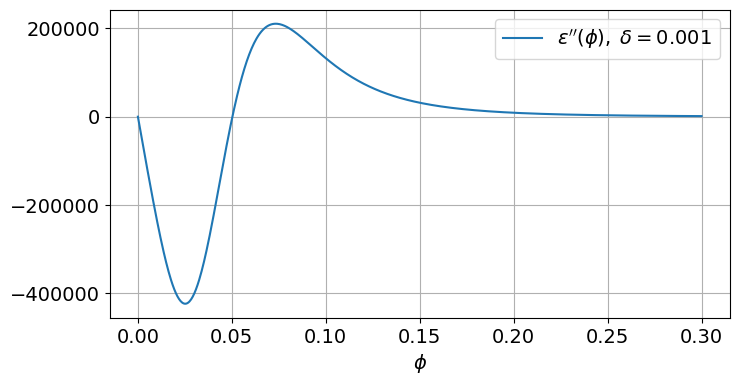
\includegraphics[width=\textwidth]{figures/eps_phi_phi.png}
	\vspace{-0.7cm}
	\caption{Typical behavior of~$\epsilon''(\phi)$ in the vicinity of~$0$.}
	\label{fig:eps_phi_phi}
\end{figure}

To proceed let us estimate extremums of~$\epsilon''(\phi)$ in the neighbourhood of~$0$.
First, find zeros of~$\epsilon'''(\phi)$. We have
\begin{equation}
	\epsilon''' = \epsilon_0 \cfrac{-6 (f')^3 + 6 (f + \delta) f' f'' - (f + \delta)^2 f'''}{(f + \delta)^4},
	\label{eq:epsilon_phi_phi_phi}
\end{equation}
form where:
$$\epsilon'''(\phi) = -6 (f')^3 + 6 (f + \delta) f' f'' - (f + \delta)^2 f''' = 0 \tcomma$$
or, taking~\eqref{eq:epsilon} into account:
$$-3 \cdot 12^2 (1 - \phi)^3 + 36 \left(4 - 3\phi + \cfrac{\delta}{\phi^3} \right)(1 - \phi)(2 - 3\phi) - \left(4 - 3 \phi + \cfrac{\delta}{\phi^3} \right)^2 (1 - 3 \phi) = 0 \tpoint$$

Let~$\delta_n \to +0$ and~$\phi_n \to +0$ such that~$\delta_n / \phi_n^3$ is bounded.
Then:
\begin{gather*}
	-3 \cdot 12^2 \cdot 1^3 + 36 \left(4 + \cfrac{\delta_n}{\phi_n^3} \right) \cdot 1 \cdot 2 - \left(4 + \cfrac{\delta_n}{\phi_n^3} \right)^2 \cdot 1 \to 0 \tcomma \\
	\left(4 + \cfrac{\delta_n}{\phi_n^3} \right)^2 - 72 \left(4 + \cfrac{\delta_n}{\phi_n^3} \right) + 3 \cdot 12^2 \to 0 \tpoint
\end{gather*}
Hence, a sequence~$4 + \delta_n / \phi_n^3$ has not more than two partial limits~$\xi_+$ and~$\xi_-$~---
which are zeros of the equation~$\xi^2 - 72 \xi + 432 = 0$.
To the first zero~$\xi_+ = 36 + 12 \sqrt{6}$ it corresponds
$$\phi_+ = \cfrac{1}{\sqrt[3]{32 + 12 \sqrt{6}}} \sqrt[3]{\delta_n} \approx \cfrac{1}{3.945} \sqrt[3]{\delta_n} \tsemicolon$$
to the second zero~$\xi_- = 36 - 12 \sqrt{6}$ it corresponds
$$\phi_- = \cfrac{1}{\sqrt[3]{32 - 12 \sqrt{6}}} \sqrt[3]{\delta_n} \approx \cfrac{1}{1.376} \sqrt[3]{\delta_n} \tpoint$$

From here it can be seen that for~$\delta \to +0$ the function~$\epsilon'''(\phi)$ has two zeros in the neighbourhood of~$0$:
\begin{equation}
  \phi_{\pm} = \cfrac{1}{\sqrt[3]{32 \pm 12 \sqrt{6}}} \sqrt[3]{\delta} [1 + o(1)] \tpoint
  \label{eq:epsilon_phi_phi_phi_roots}
\end{equation}

We now estimate~$\epsilon''(\phi)$ at~$\phi_{\pm}$  for~$\delta \to +0$. Let~$\phi = (1 / c) \sqrt[3]{\delta}$, $c \in \Real$.
Then:
$$\epsilon'' = \epsilon_0 \cfrac{24 c^5 (8 - c^3)}{(4 + c^3)^3} \delta^{-5 / 3} [1 + o(1)],$$
and:
\begin{equation}
  \epsilon''(\phi_+) \approx -4.378 \epsilon_0 \delta^{-5 / 3}; \quad \epsilon''(\phi_-) \approx 2.216 \epsilon_0 \delta^{-5 / 3} \tpoint
  \label{est:epsilon_phi_phi_bounds}
\end{equation}
The derived estimates are shown as black dashed lines on Fig.~\ref{fig:eps_phi_phi_multiplied}.

\begin{figure}[!t]
	\centering
	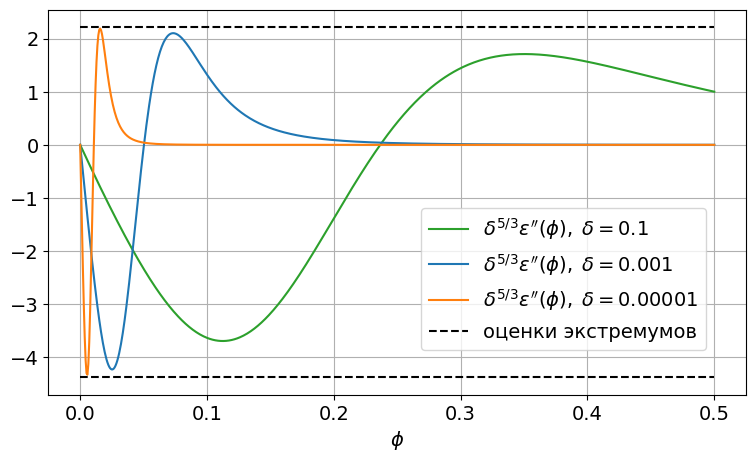
\includegraphics[width=\textwidth]{figures/eps_phi_phi_multiplied.png}
	\caption{Qualitative behavior of~$\delta^{5 / 3} \epsilon''(\phi)$ for small values of~$\delta$.}
	\label{fig:eps_phi_phi_multiplied}
\end{figure}

Now, to derive new stability estimate we consider equation~\eqref{eq:spectral} at~$\phi = \phi_+$.
Note that~$\epsilon''(\phi_+) \approx -4.4 \epsilon_0 \delta^{-5 / 3}$.
The term inside braces in~\eqref{eq:spectral} is negative since
$\delta$ is small and~$\epsilon''(\phi_+)$ is negative and large in its absolute value.
Therefore~$f''(\phi_+) > 0$ can be estimated as~$0$~--- such estimate makes inequality stronger.
Then from inequality~\eqref{eq:spectral} it follows that 
$$\lambda(\theta) = 1 + m \tau \left( -\cfrac{2.2 K_\Phi^2 \epsilon_0}{\delta^{5 / 3}} - \cfrac{2 \Gamma}{h^2} \sin^2 \cfrac{\theta}{2} \right) \tpoint$$
Condition~$|\lambda(\theta)| \leqslant 1$ is satisfied for an arbitrary~$\theta$, if and only if
\begin{equation}
  \tau \leqslant \cfrac{1}{m} \left( \cfrac{1.1 K_\Phi^2 \epsilon_0}{\delta^{5 / 3}} + \cfrac{\Gamma}{h^2} \right)^{-1} \tpoint
  \label{cond:spectral_better_theoretical}
\end{equation}

Numerical experiments described in the next sections indicates that
more strong version of the estimate~\eqref{cond:spectral_better_theoretical} is also valid
(note the doubled denominator):
%
\begin{equation}
  \tau \leqslant \cfrac{1}{2m} \left( \cfrac{K_\Phi^2 \epsilon_0}{\delta^{5 / 3}} + \cfrac{\Gamma}{h^2} \right)^{-1} \tpoint
  \label{cond:spectral_better}
\end{equation}

Finally, more simple estimate not weaker then~\eqref{cond:spectral_better} is:
\begin{equation}
  \tau \leqslant \cfrac{1}{4m} \min \left(\cfrac{\delta^{5 / 3}}{K_\Phi^2 \epsilon_0}, \; \cfrac{h^2}{\Gamma} \right) \tpoint
  \label{cond:spectral_better_simpler}
\end{equation}

Note that the derived stability estimate~\eqref{cond:spectral_better}
for finite-difference scheme~\eqref{sch:transition},\eqref{sch:borders}
includes all the parameters of the equation~\eqref{eq:one_dim}, except~$l$.
Notably, this is the only parameter of the model which has somehow artificial nature and can not be
related directly to the underlying physics.

\endinput
% EOF

%!TEX root = ../main.tex

\section{Вычислительный эксперимент}

Была написана программа, реализующая разностную схему \eqref{sch:all}.

Все предыдущие рассуждения были универсальны для плоского, цилиндрического и сферического случаев, насколько это возможно. Все три случая моделируются одной и той же программой, принимающей $k = \overline{0, 2}$ как параметр.

Зададим параметры модели:
$$\epsilon_0 = 0.2, \; \delta = 0.04, \; l = 1.0, \; \Gamma = 1.0, \; m = 0.5 \tpoint$$

Пусть $R = 5$. По виду графиков будет понятно, что для использованного набора параметров такое $R$ достаточно велико.

Выберем число ячеек $n = 300$ при $\alpha = 0$ и $n = 150$ иначе. Шаг по пространству~$h$, соответственно, равен $1/30 \approx 0.0333$ либо $1/60 \approx 0.0167$. При этом придется брать шаг по времени $\tau = 5 \cdot 10^{-7}$. Если шаг по времени кратно больше, то схема оказывается неустойчива и программа завершается с ошибкой переполнения (в данных возникает значение NaN). Как и ожидалось, $p$-лапласиан и билапласиан (особенно) требуют относительно малых шагов по времени.

Выбор начальных условий не имеет значения. Пусть, например, значения $0$ и $1$ гладко соединяются ветвью синусоиды: $\widetilde{\phi}_i^0 = \sin[(h/2 + ih) \pi / 2], \; h/2 + ih < 1$; далее все значения равны $1$.

Будем останавливать расчет, когда вектор <<воздействия>> на систему достаточно мал, а именно:
$$\max\limits_{i = 0}^n \cfrac{\widetilde{\phi}_i^{j + 1} - \widetilde{\phi}_i^j}{m} < 10^{-9} \tpoint$$
Все конфигурации модели достигли названного условия не более чем через $7.4$ единицы времени.

Результаты вычислений изображены на рис. \ref{fig:result_volumes} и \ref{fig:result_volumes_p} (случай 1 из описания разностной схемы), рис. \ref{fig:result_volumes_bi} (случай 2), рис. \ref{fig:result_volumes_cyl_p} (случай 3), рис. \ref{fig:result_volumes_cyl_bi} (случай 4), рис.~\ref{fig:result_volumes_sph_p} (случай~5). Графики функций показаны до зримого момента выхода на примерно постоянное значение $1$, после чего они в действительности продолжаются до $R = 5$. Графики состоят из соединенных значений средних $\widetilde{\phi}_i^j$, размещенных в серединах ячеек; вблизи~$0$ к ним добавлено несколько значений приближающей функции $g^{(a)}$, имеющей особенность в $0$, если того требует случай задачи.

\begin{figure}[!tp]
	\centering
	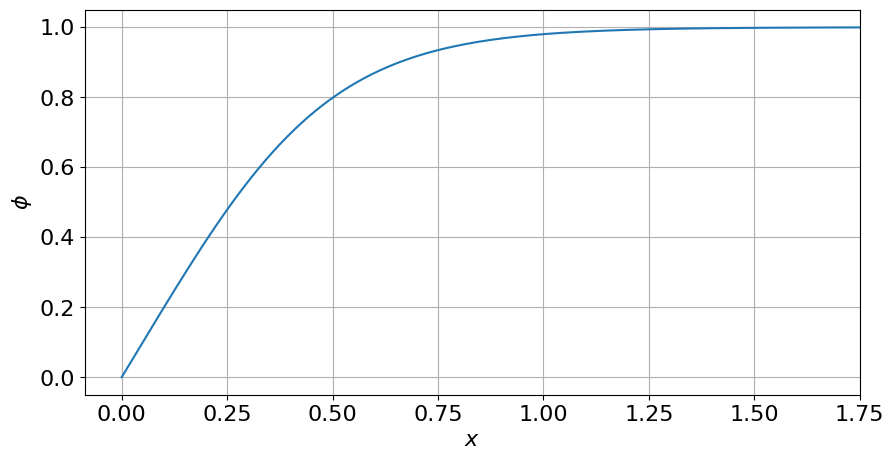
\includegraphics[width=0.89\textwidth]{figures/result_volumes.png}
	\vspace{-0.3cm}
	\caption{Решение $\phi$ в плоском случае при $\alpha = 0, \; \beta = 0$.}
	\label{fig:result_volumes}
	\vspace{0.5cm}

	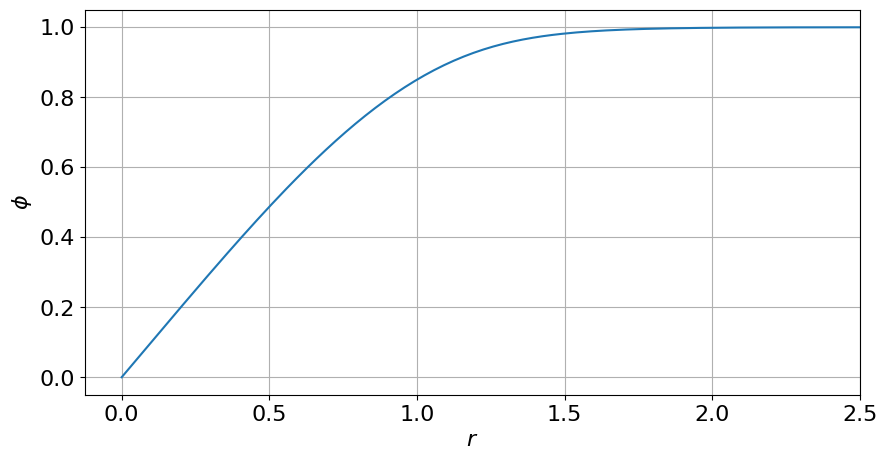
\includegraphics[width=0.89\textwidth]{figures/result_volumes_p.png}
	\vspace{-0.3cm}
	\caption{Решение $\phi$ в плоском случае при $\alpha = 0, \; \beta = 1$.}
	\label{fig:result_volumes_p}
	\vspace{0.5cm}
	
	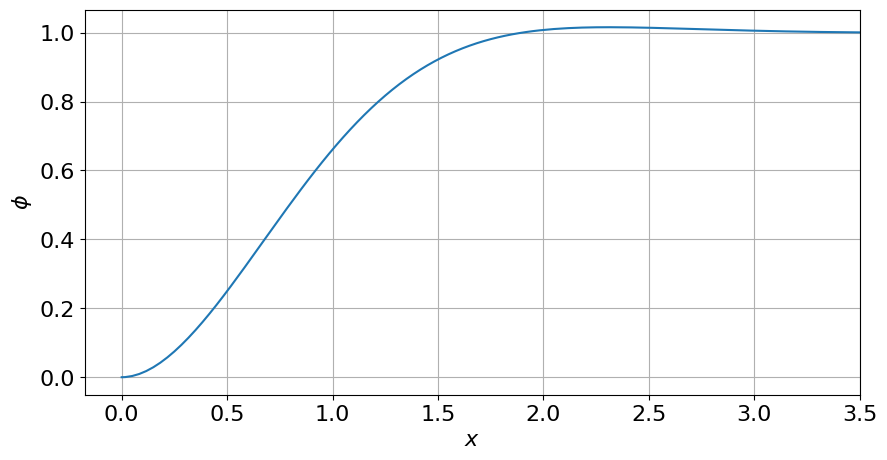
\includegraphics[width=0.89\textwidth]{figures/result_volumes_bi.png}
	\vspace{-0.3cm}
	\caption{Решение $\phi$ в плоском случае при $\alpha = 1, \; \beta = 0$.}
	\label{fig:result_volumes_bi}
\end{figure}

\begin{figure}[!tp]
	\centering
	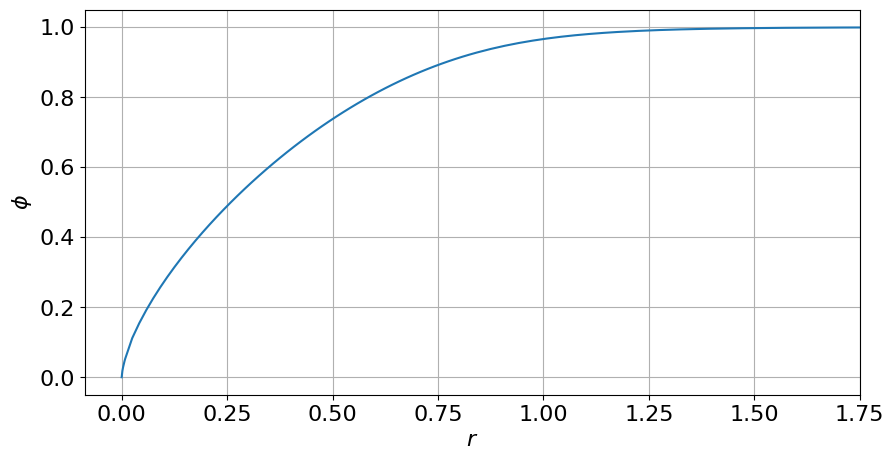
\includegraphics[width=0.89\textwidth]{figures/result_volumes_cyl_p.png}
	\vspace{-0.3cm}
	\caption{Решение $\phi$ в цилиндрическом случае при $\alpha = 0, \; \beta = 1$.}
	\label{fig:result_volumes_cyl_p}
	\vspace{0.5cm}

	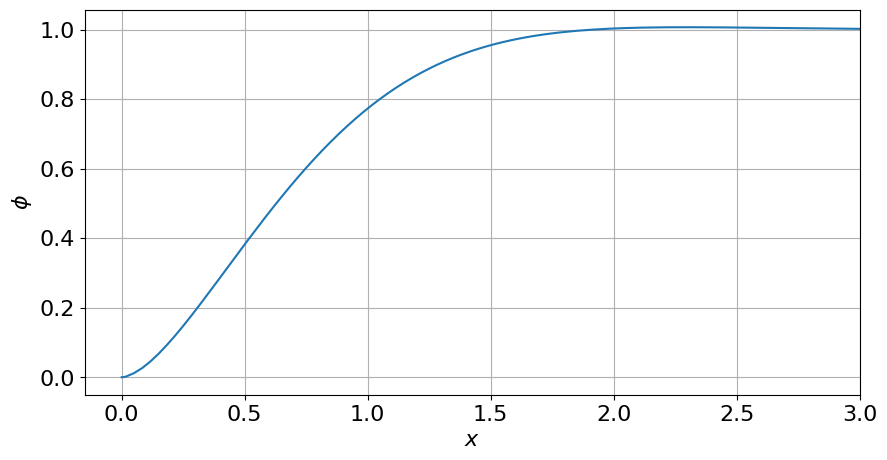
\includegraphics[width=0.89\textwidth]{figures/result_volumes_cyl_bi.png}
	\vspace{-0.3cm}
	\caption{Решение $\phi$ в цилиндрическом случае при $\alpha = 1, \; \beta = 0$.}
	\label{fig:result_volumes_cyl_bi}
	\vspace{0.5cm}
	
	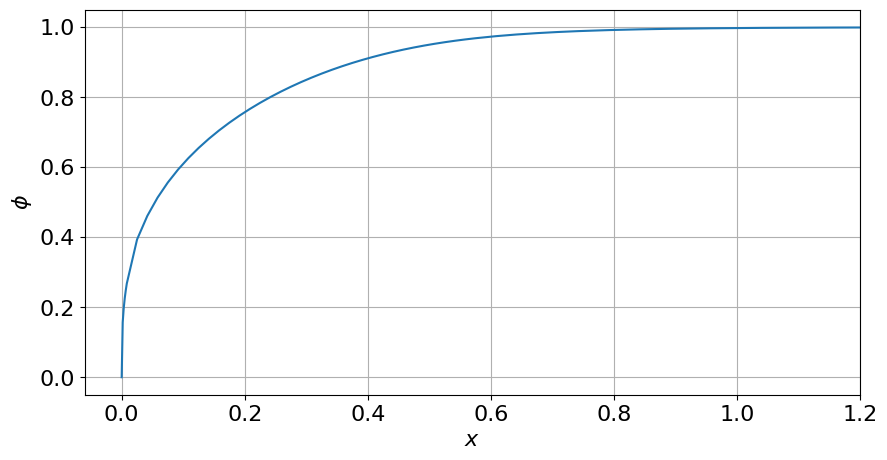
\includegraphics[width=0.89\textwidth]{figures/result_volumes_sph_p.png}
	\vspace{-0.3cm}
	\caption{Решение $\phi$ в сферическом случае при $\alpha = 0, \; \beta = 1$.}
	\label{fig:result_volumes_sph_p}
\end{figure}

Отметим, что если в уравнения входит билапласиан ($\alpha \neq 0$), то функция $\phi$ может быть не монотонной и в некоторых точках превышать значение $1$ (см. рис. \ref{fig:result_volumes_bi}, \ref{fig:result_volumes_cyl_bi}). В работе \cite{zipunova_higher_codimension} это было отмечено и указано, что монотонность $\phi$ следует ожидать при достаточно малых $\alpha$.

Итак, эксперимент подтверждает, что, несмотря на некоторую громоздкость формулировок, предложенная модификация метода конечных объемов позволяет эффективно моделировать решение $\phi$, даже если на границе области оно имеет особенность.

%!TEX root = ../main.tex

\section{Заключение}

Настоящая работа продолжает исследование, начатое в статье \cite{zipunova_higher_codimension}. Как было отмечено ее авторами, исследование это хотя и проводится для конкретной задачи, но, вероятно, затрагивает вопросы, содержащиеся в методе диффузной границы как таковом. Суть этих вопросов в том, позволяют ли уравнения среды с диффузной границей в своей <<классической>> редакции адекватно описывать включения, по своей природе являющиеся объектами высшей коразмерности. В качестве возможного ответа авторы работы \cite{zipunova_higher_codimension} предлагают определенного вида обобщение исходной модели.

Целью настоящей работы было численно исследовать упомянутое обобщение. В этом достигнуты определенные успехи. С помощью модификации метода конечных объемов преодолены трудности, связанные с необходимостью задавать граничные условия на множествах коразмерности 2 и 3 в трехмерном пространстве и с наличием у функции-решения  особенности в точках этих множеств. Указанный подход существенно не привязан к рассматриваемой модели -- в дальнейшем он может быть использован и в других задачах.

В некоторых случаях при построении разностной схемы возникали фундаментальные препятствия: оказывалось, что необходимых базисных функций попросту не существует. На основании этого выдвинута гипотеза, что в указанных случаях рассматриваемая дифференциальная задача поставлена некорректно и не имеет решения. Рассуждения вполне согласуется с теоретическими результатами работы \cite{zipunova_higher_codimension}. В будущем возможно строгое обоснование представленной гипотезы.

\clearpage
\printbibliography[
	heading=bibintoc
]

\clearpage
\tableofcontents

\end{document}

%%%%%%%%%%%%%%%%%%%%%%%%%%%%%%%%%%%%%%%%%%%%%%%%%%%%%%%%%%%%%%%%%%%%%%%%%%%%%%%%